\documentclass{beamer}

% TODO: print out https://www.fuzzingbook.org/code/Intro_Testing.py

\usetheme{Boadilla}

%\includeonlyframes{current}

\usepackage{times}
\usefonttheme{structurebold}
\usepackage{listings}

\usepackage{pgf}
\usepackage{tikz}
\usepackage{alltt}
\usepackage[normalem]{ulem}
\usetikzlibrary{arrows}
\usetikzlibrary{automata}
\usetikzlibrary{shapes}
\usepackage{amsmath,amssymb}
\usepackage{rotating}
\usepackage{ulem}

\usetikzlibrary{arrows,automata,shapes}
\tikzstyle{block} = [rectangle, draw, fill=blue!20, 
    text width=5em, text centered, rounded corners, minimum height=2em]
\tikzstyle{bt} = [rectangle, draw, fill=blue!20, 
    text width=4em, text centered, rounded corners, minimum height=2em]

\lstdefinelanguage{JavaScript}{
  keywords={typeof, new, true, false, catch, function, return, null, catch, switch, var, if, in, while, 
do, else, case, break},
  keywordstyle=\color{blue}\bfseries,
  ndkeywords={class, export, boolean, throw, implements, import, this},
  ndkeywordstyle=\color{darkgray}\bfseries,
  identifierstyle=\color{black},
  sensitive=false,
  comment=[l]{//},
  morecomment=[s]{/*}{*/},
  commentstyle=\color{purple}\ttfamily,
  stringstyle=\color{red}\ttfamily,
  morestring=[b]',
  morestring=[b]''
}

%\setbeamercovered{dynamic}
\setbeamertemplate{footline}[page number]{}
\setbeamertemplate{navigation symbols}{}
\usefonttheme{structurebold}

\title{Software Testing, Quality Assurance \& Maintenance---Lecture 4}
\author{Patrick Lam\\University of Waterloo}
\date{January 15, 2025}

\colorlet{redshaded}{red!25!bg}
\colorlet{shaded}{black!25!bg}
\colorlet{shadedshaded}{black!10!bg}
\colorlet{blackshaded}{black!40!bg}

\colorlet{darkred}{red!80!black}
\colorlet{darkblue}{blue!80!black}
\colorlet{darkgreen}{green!80!black}

\newcommand{\rot}[1]{\rotatebox{90}{\mbox{#1}}}
\newcommand{\gray}[1]{\mbox{#1}}

\newenvironment{changemargin}[1]{% 
  \begin{list}{}{% 
    \setlength{\topsep}{0pt}% 
    \setlength{\leftmargin}{#1}% 
    \setlength{\rightmargin}{1em}
    \setlength{\listparindent}{\parindent}% 
    \setlength{\itemindent}{\parindent}% 
    \setlength{\parsep}{\parskip}% 
  }% 
  \item[]}{\end{list}}



\begin{document}

\usebackgroundtemplate{\tikz\node[opacity=0.1]{
\includegraphics[width=\paperwidth]{L02/07172_about_banmochi_ishi_strength_and_grip_testing.JPG}};}
\begin{frame}
  \titlepage
\end{frame}

\part{When to stop? \\ Idea 2: Mutation Analysis}
\begin{frame}
  \partpage
\end{frame}

\usebackgroundtemplate{\tikz\node[opacity=0.3]{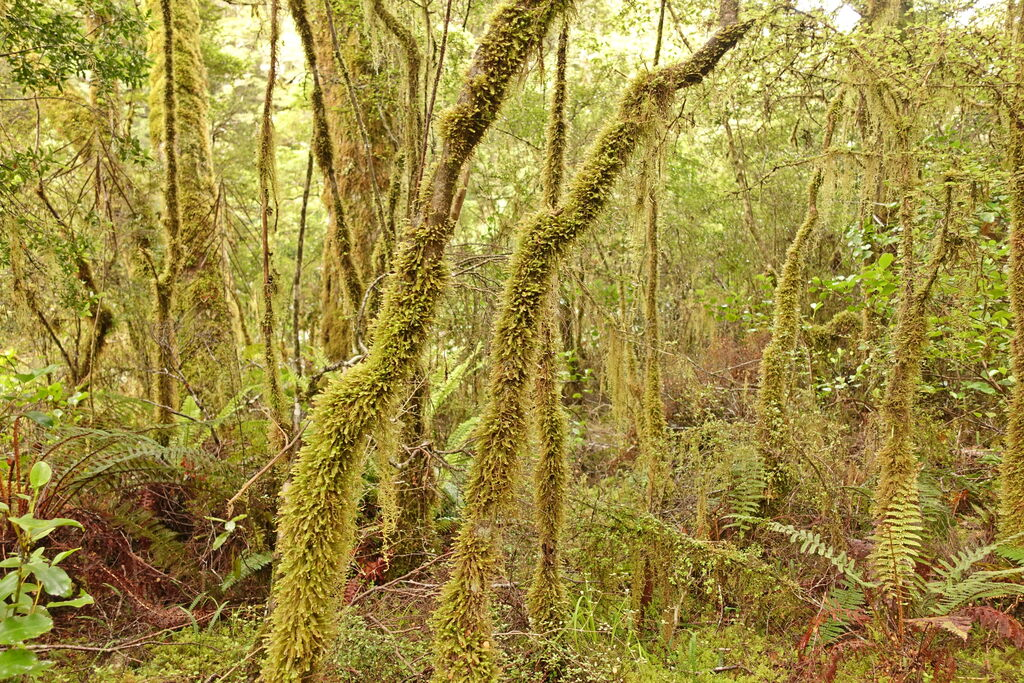
\includegraphics[width=\paperwidth]{L03/09038_lots_of_moss_v1.JPG}};}
\begin{frame}
  \frametitle{How many tests?}
  \Large
  \begin{changemargin}{2em}
    Do you have enough tests? How do you know?\\[1em]

    Let's fuzz the test suite.\\
    ~~ How? Modifying the program and seeing if the test suite notices.
  \end{changemargin}
\end{frame}

\usebackgroundtemplate{\tikz\node[opacity=0.3]{
\includegraphics[width=\paperwidth]{L04/20241110_001424746_blackbird.jpg}};}
\begin{frame}
  \frametitle{Mutants}
  \Large
  \begin{changemargin}{2em}
    A \alert{mutant} is a modified version of the program being tested.\\[1em]
    Usually we change an operator or identifier:
    \[ x + 5 \Rightarrow x - 5 \]
    
  \end{changemargin}
\end{frame}

\usebackgroundtemplate{}
\begin{frame}
  \frametitle{Killing Mutants}
  \Large
  \begin{changemargin}{2em}
    The test suite should fail on the mutant. \\
    Then the mutant is \alert{killed}.\\[1em]

    Remember: arrange, act, assert.\\
    Mutant might trigger errors during act;\\
    or it may detect different output during assert.
  \end{changemargin}
\end{frame}

\begin{frame}[fragile]
  \frametitle{Example Mutants}
  \begin{changemargin}{2em}
    Use language grammar to create mutants (code/L04/minval.c).\\[1em]
  \end{changemargin}
  \small
\begin{minipage}[t]{.4\textwidth}
\begin{alltt}
// original
int min(int a, int b)
\{
  int minVal;
  minVal = a;

  if (b < a) \{


    minVal = b;



  \}
  return minVal;
\}
\end{alltt}
\end{minipage} \begin{minipage}[t]{.4\textwidth}
\begin{alltt}
// with mutants
int min(int a, int b)
\{
  int minVal;
  minVal = a;
  minVal = b;               // \(\Delta 1\)
  if (b < a) \{
  if (b > a) \{              // \(\Delta 2\)
  if (b < minVal) \{         // \(\Delta 3 \)
    minVal = b;
    BOMB();                 // \(\Delta 4\)
    minVal = a;             // \(\Delta 5\)
    minVal = failOnZero(b); // \(\Delta 6\)
  \}
  return minVal;
\}
\end{alltt}
\end{minipage}
  
\end{frame}

\begin{frame}[fragile]
  \frametitle{Testing on the mutants}

  \begin{changemargin}{2em}
    Here's a test suite. How do the mutants do? \\[1em]
\begin{tabular}{lcccccc}
  & $\Delta$ 1 & $\Delta$ 2 & $\Delta$ 3 & $\Delta$ 4 & $\Delta$ 5 & $\Delta$ 6\\ 
  $\langle a = 0, b = 1, \mathrm{exp} = 0 \rangle$   & kill & & -- \\
  $\langle a = 1, b = 0, \mathrm{exp} = 0 \rangle$   & --   & & -- \\
  $\langle a = 1, b = 1, \mathrm{exp} = 1 \rangle$   &      & & -- \\
  $\langle a = 1, b = 349, \mathrm{exp} = 1 \rangle$ &      & & -- \\
\end{tabular}

~\\
Observe: $\Delta 3$ not killable.
    
  \end{changemargin}
\end{frame}

\begin{frame}
  \frametitle{Key idea for Mutation Analysis}
  \Large
  \begin{changemargin}{2em}
    Idea: use mutation analysis to evaluate test suite quality/improve test suites.\\[1em]
    Good test suites ought to be effective at killing mutants.
  \end{changemargin}

\end{frame}


\begin{frame}
  \frametitle{Why should this work? (1/2)}

    \Large
    \begin{changemargin}{2em}
      \alert{Competent Programmer Hypothesis}: \\
      \hspace*{2em}programmers usually are almost right,\\
      \hspace*{2em}except for ``subtle, low-level faults''.\\[1em]
      Mutation analysis tries to mimic this. (Exceptions?)
  \end{changemargin}

\end{frame}

\begin{frame}
  \frametitle{Why should this work? (2/2)}

    \Large
    \begin{changemargin}{2em}
      \alert{Coupling Effect Hypothesis}: \\
      \hspace*{2em}complex faults are the result of \\
      \hspace*{2em} simple faults combining.\\[1em]
      Hence, detecting all simple faults will detect many complex faults.\\[2em]

      Implication: test suites that are good at ensuring program quality also good at killing mutants.
      
  \end{changemargin}

\end{frame}

\usebackgroundtemplate{\tikz\node[opacity=0.1]{
\includegraphics[width=\paperwidth]{L04/0207_gold_mask.JPG}};}
\begin{frame}
  \frametitle{Mutation analysis in context}

  \begin{changemargin}{2em}
    Hard to apply by hand, and automation is complicated.\\[1em]
    Mutation is a ``gold standard'' \\
    \hspace*{2em} against which to test other testing criteria.\\[1em]
    Consider test suite $T$ which ensures statement coverage. \\
    What does mutation analysis say about $T$?
\end{changemargin}
\end{frame}

\usebackgroundtemplate{}

\begin{frame}
  \frametitle{Using Mutation Analysis}

  \Large
  \begin{changemargin}{2em}
    Three steps:
    \begin{enumerate}
    \item Generate mutants (usually with a tool)
    \item Execute mutants (computationally expensive)
    \item Classify (manual)
    \end{enumerate}
    ~\\
    Then, create new test cases to kill remaining mutants.
  \end{changemargin}
  
\end{frame}

\begin{frame}[fragile]
  \frametitle{Mutation Analysis Diagram}
  \begin{center}
    \small
\resizebox{\textwidth}{.8\textheight}{%
\begin{tikzpicture}[->,>=stealth',shorten >=1pt,auto,node distance=3cm,
                    text width=4em,
                    semithick,initial text=]
  \node[text width=6em] (p) {Program $P$};
  \node[block,right of=p] (create) {Create mutants $m$};
  \node[block,right of=create] (elim) {Eliminate known-equivalent mutants};
  \node[block,right of=elim] (gen) {Generate test cases $T$};
  \node[block,right of=gen] (runTonP) {Run $T$ on $P$};
  \node[block,below of=runTonP,yshift=2em] (runTonM) {Run $T$ on all $M$};
  \node[block, below of=runTonM,yshift=2em] (filter) {Filter bogus mutants};
  \node[shape=ellipse, text centered, fill=blue!20, draw, text width=5em, left of=filter] (enough) {Enough mutants killed?};
  \node[block, left of=enough] (findThreshold) {Define threshold};
  \node[shape=ellipse, text centered, fill=blue!20, draw, text width=5em, below left of=enough,xshift=-10em] (correct) {Output of $p$ on $T$ correct?};
  \node[block, below of=correct,yshift=2em] (done) {Done};
  \node[block, below of=p,yshift=2em] (fixP) {Fix $P$};

  \path (p) edge node {} (create)
        (create) edge node {} (elim)
        (elim) edge node {} (gen)
        (gen) edge node {} (runTonP)
        (runTonP) edge node {} (runTonM)
        (runTonM) edge node {} (filter)
        (filter) edge node {} (enough)
        (findThreshold) edge node {} (enough)
        (correct) edge node {yes} (done)
        (fixP) edge node {} (p);
  \draw (correct) -| node[xshift=3em,yshift=2em] {no} (fixP); % no
  \draw (enough.north) -- node[xshift=2.5em] {no} (gen);
  \draw (enough) |- node[near start] {yes} (correct);
\end{tikzpicture}
}
\end{center}

\end{frame}


  \end{document}
